%-*- coding: UTF-8 -*-
% Customizing.tex
%
\documentclass[UTF8]{ctexart}
\usepackage{geometry}
\geometry{a4paper, centering, scale=0.8}
\usepackage{minted}
\usepackage{graphicx}   % 为了使用插图功能
\usepackage{hyperref}

\title{\heiti 第6章 \quad \LaTeX 的私人订制}
\author{\kaishu Du Ang \\ \texttt{du2ang233@gmail.com} }
\date{\today}

% Define a newcommand to show visible space
\newcommand\Vtextvisiblespace[1][.3em]{%
  \mbox{\kern.06em\vrule height 1ex}%
  \vbox{\hrule width#1}%
  \hbox{\vrule height 1ex}}


\begin{document}
\maketitle

\tableofcontents

\newpage

之前学到的一些命令看似都够用了,但是它们的输出的效果有时并不是特别好看。而且有的时候,\LaTeX 提供的命令或环境并不能满
足我们的要求。试想:我要如何制作一个简单但像样的毕业论文/书籍/简历模板,每次都可以直接套用,而不是再在导言区写一堆代码?

这一章的内容可以帮我们实现这一目标,让我们编写可重复利用的模块——宏包和文档类,并在其中自己定义命令和环境,让 \LaTeX 产
生不同于默认的输出。

\section{自定义命令、环境、宏包和文档类}
\subsection{定义新命令}
定义新命令:
\begin{minted}{LaTeX}
    \newcommand{name}[num]{definition}
\end{minted}

该命令需要两个基本的参数:新命令的名字 \emph{name} 和 新命令的定义 \emph{definition}。可选参数 \emph{num} 可以
指定新命令的参数数目(最多9个)。如果不写 \emph{num} 参数,默认为0,表示新命令没有参数。

示例 1 定义了一个新命令 \mintinline{LaTeX}{\tnss},是“The Not So Short Introduction to \LaTeXe” 的缩写。

示例代码1:
\begin{minted}{LaTeX}
    \newcommand{\tnss}{The not so Short Introduction to \LaTeXe}
    % in the document body:
    This is ``\tnss'' \ldots{} ``\tnss''
\end{minted}

示例输出1:
\begin{quote}
    \newcommand{\tnss}{The not so Short Introduction to \LaTeXe}
    % in the document body:
    This is ``\tnss'' \ldots{} ``\tnss''
\end{quote}

示例 2 定义了包含参数的命令。使用定义的命令的时候,在 \texttt{\#1} 的位置指定参数。如果需要定义更多的参数,使用
\texttt{\#2}、\texttt{\#3},以此类推。

示例代码2:
\begin{minted}{LaTeX}
    \newcommand{\txsit}[2]{This is the \emph{#1} #2 Introduction to \LaTeXe}
    % in the document body:
    \begin{itemize}
        \item \txsit{not so}{short}
        \item \txsit{very}{long}
    \end{itemize}
\end{minted}

示例输出2:
\begin{quote}
    \newcommand{\txsit}[2]{This is the \emph{#1} #2 Introduction to \LaTeXe}
    % in the document body:
    \begin{itemize}
        \item \txsit{not so}{short}
        \item \txsit{very}{long}
    \end{itemize}
\end{quote}

\LaTeX 不允许定义一个与现有命令重名的命令。如果要修改命令定义,使用 \mintinline{LaTeX}{\renewcommand} 命令。它
的用法与 \mintinline{LaTeX}{\newcommand} 相同。

在某些情况下,可能会用到 \mintinline{LaTeX}{\providecommand} 命令。在命令不存在时,它相当于
\mintinline{LaTeX}{\newcommand};在命令已经存在时,仍沿用原来已存在的定义。

\subsection{定义新环境}
和 \mintinline{LaTeX}{\newcommand} 命令类似,可以通过 \mintinline{LaTeX}{\newenvironment} 命令来定义环境:
\begin{minted}{LaTeX}
    \newenvironment{name}[num]{before}{after}
\end{minted}

同样地,\mintinline{LaTeX}{\newenvironment} 有一个可选的参数 \emph{num}。\emph{before} 参数中的内容将在此环
境包含的文本之前处理,\emph{after} 参数中的内容将在遇到 \mintinline{LaTeX}|\end{name}| 命令时处理。

示例代码:
\begin{minted}{LaTeX}
    \newenvironment{king}
        {\rule{1ex}{1ex} \hspace{\stretch{1}}}
        {\hspace{\stretch{1}} \rule{1ex}{1ex}}
    % in the document body:
    \begin{king}
        My humble subjects \ldots
    \end{king}
\end{minted}

示例输出:
\begin{quote}
    \newenvironment{king}
        {\rule{1ex}{1ex} \hspace{\stretch{1}}}
        {\hspace{\stretch{1}} \rule{1ex}{1ex}}
    % in the document body:
    \begin{king}
        My humble subjects \ldots
    \end{king}
\end{quote}

\emph{num} 参数的用法和 \mintinline{LaTeX}{\newcommand} 命令相同。同样,也不能定义一个现有的环境,如果想修改某
个现有的环境,使用 \mintinline{LaTeX}{\renewenvironment} 命令,语法和 \mintinline{LaTeX}{\newenvironment}
相同。

上面示例中的 \mintinline{LaTeX}{\rule}、\mintinline{LaTeX}{\stretch} 和 \mintinline{LaTeX}{\hspace} 命
令后面会介绍。

\subsection{多余的空格}
在定义一个新环境的时候,很容易会有多余的空格“悄悄溜进来”。这样的小瑕疵有些时候却很致命,例如我们想创建一个没有缩进的标
题环境、并且希望紧跟这个环境后面的段落也不要缩进的时候。\mintinline{LaTeX}{\ignorespaces} 命令会忽略环境开始部分
的所有空格。想在环境结束后不留空格有点麻烦,可以用 \linebreak[6] \mintinline{LaTeX}{\ignorespacesafterend} 命令,它的作用是在
环境的“end”之后执行 \mintinline{LaTeX}{\ignorespaces}。

示例代码:
\begin{minted}{LaTeX}
    \newenvironment{simple}
        {\noindent}
        {\par\noindent} % \par ends the paragraph
    % in the document body:
    \begin{simple}
        See the space \\ to the left.
    \end{simple}
    Same \\ here.

    \newenvironment{correct}
        {\noindent\ignorespaces}
        {\par\noindent\ignorespacesafterend}
    % in the document body:
    \begin{correct}
        No space \\ to the left
    \end{correct}
    Same \\ here.
\end{minted}

示例输出:
\begin{quote}
    \newenvironment{simple}
        {\noindent}
        {\par\noindent} % \par ends the paragraph
    % in the document body:
    \begin{simple}
        See the space \\ to the left.
    \end{simple}
    Same \\ here.

    \newenvironment{correct}
        {\noindent\ignorespaces}
        {\par\noindent\ignorespacesafterend}
    % in the document body:
    \begin{correct}
        No space \\ to the left
    \end{correct}
    Same \\ here.
\end{quote}

\subsection{\LaTeX 的命令行参数}
如果用的是类 Unix 操作系统,就可能会用 Makefile 来构建 \LaTeX 项目,然后就可以用不同的命令行参数使使同一份文档编译
出不同的版本。如果在文档中加入下面的代码:
\begin{minted}{LaTeX}
    \usepackage{ifthen}
    \ifthenelse{\equal{\blackandwhite}{true}}{
        % "black and white" mode; do something...
    }{
        % "color" mode; do something different...
    }
\end{minted}

然后利用下面的命令调用 \LaTeX:
\begin{minted}{LaTeX}
    latex '\newcommand{blackandwhite}{true}\input{test.tex}'
\end{minted}

首先 \mintinline{LaTeX}{\blackandwhite} 命令会被定义,然后真实的文件会被读取。如果将
\mintinline{LaTeX}{\blackandwhite} 设置为 false,文档就会输出彩色版本。

\subsection{定义新宏包}
如果定义了很多的新环境和新命令,文档的导言区就会很长。这时,就可以定义一个 \LaTeX 宏包来包含所有新环境和新命令的定义。
需要时,再在文档中通过 \mintinline{LaTeX}{\usepackage} 命令调用。

如果想要自定义一个宏包,基本的工作是要将原来写在文档导言区的很长的内容拷贝到一个 \texttt{.sty} 文件中,并且需要在文件
最前面加上 \mintinline{LaTeX}|\ProviedesPackage{package name}| 命令,这个命令可以在多次包含宏包的问题提示错
误。其中,\emph{package name} 要和我们定义的宏包名相同。

示例代码:
\begin{minted}{LaTeX}
    % Demo Package by Tobias Oetiker
    \ProvidesPackage{demopack}
    \newcommand{\tnss}{The not so Short Introduction to \LaTeXe}
    \newcommand{\txsit}[1]{The \emph{#1} Short Introduction to \LaTeXe}
    \newenvironment{king}{\begin{quote}}{\end{quote}}
\end{minted}

如果想进一步把各种宏包的功能汇总到一个文件里,而不是在文档的导言区罗列一大堆宏包的话,\LaTeX 允许我们在自己编写的宏包
中调用其他宏包,命令为 \mintinline{LaTeX}{\RequirePackage},用法和 \mintinline{LaTeX}{\usepackage} 一致:
\begin{minted}{LaTeX}
    \RequirePackage[options]{package name}
\end{minted}

\subsection{定义新的文档类}
再进一步,如果想编写自己的文档类,如论文模板等,问题就稍稍麻烦一些了。首先,要把自定义的文档类文件以 \texttt{.cls} 作
为扩展名,开头使用 \mintinline{LaTeX}{\ProvidesClass} 命令:
\begin{minted}{LaTeX}
    \ProvidesClass{class name}
\end{minted}

同样地,\emph{class name} 也要和文档类的文件名一致。

但是有了上述命令和之前学到的一些命令,还不足以完成一个文档类的编写。因为诸如 \mintinline{LaTeX}{\chapter}、
\mintinline{LaTeX}{\section} 等等许多命令都是在文档类中定义的。事实上,许多时候我们只需要像调用宏包那样调用一个基
本的文档类,这样可以省去许多不必要的麻烦。在文档类中使用其他文档类的命令是 \mintinline{LaTeX}{\LoadClass},用法和
\mintinline{LaTeX}{\documentclass} 十分相像:
\begin{minted}{LaTeX}
    \LoadClass[options]{package name}
\end{minted}

\section{字体和字号}
\subsection{改变字体的命令}
\LaTeX 默认会根据文档的逻辑结构(章节、脚注等)自动选择适当的字体和字号。但是如果我们想自己手动地改变它们,这时就
可以用表~\ref{tab:fonts} 和表~\ref{tab:sizes}。每种字体的真实大小是由文档类和它的设置决定的。
表~\ref{tab:pointsizes} 展示了这些命令的绝对磅值,是由标准文档类定义的。

示例代码:
\begin{minted}{LaTeX}
    {\small The smal and \textbf{bold} Romans ruled}
    {\Large all of great big \textit{Italy}.}
\end{minted}

示例输出:
\begin{quote}
    {\small The smal and \textbf{bold} Romans ruled}
    {\Large all of great big \textit{Italy}.}
\end{quote}

\LaTeXe 的一个重要特点是字体的属性是独立的。意思是,如果一段文字事先被设置了粗体或斜体,后来又改变了它的字号或者字体,
它会在原来粗体或斜体设置的基础上变化。

在数学模式中,使用改变字体命令可以暂时地退出数学模式,并且输入一些正常的字体。如果想换成另一种数学排版字体,需要使用到
表~\ref{tab:mathfonts} 中的一些命令。

\begin{table}[!bp]
\centering
\caption{字体命令} \label{tab:fonts}
%
% Alan suggested not to tell about the other form of the command
% eg \verb|\sffamily| or \verb|\bfseries|. This seems a good thing to me.
%
\begin{tabular}{@{}rl@{\qquad}rl@{}}
\mintinline{LaTeX}|\textrm{...}|        &      \textrm{roman}&
\mintinline{LaTeX}|\textsf{...}|        &      \textsf{sans serif}\\
\mintinline{LaTeX}|\texttt{...}|        &      \texttt{typewriter}\\[6pt]
\mintinline{LaTeX}|\textmd{...}|        &      \textmd{medium}&
\mintinline{LaTeX}|\textbf{...}|        &      \textbf{bold face}\\[6pt]
\mintinline{LaTeX}|\textup{...}|        &       \textup{upright}&
\mintinline{LaTeX}|\textit{...}|        &       \textit{italic}\\
\mintinline{LaTeX}|\textsl{...}|        &       \textsl{slanted}&
\mintinline{LaTeX}|\textsc{...}|        &       \textsc{Small Caps}\\[6pt]
\mintinline{LaTeX}|\emph{...}|          &            \emph{emphasized} &
\mintinline{LaTeX}|\textnormal{...}|    &    \textnormal{document} font
\end{tabular}
\end{table}

\begin{table}[!bp]
\centering
\caption{字号命令} \label{tab:sizes}
\begin{tabular}{@{}ll}
\mintinline{LaTeX}|\tiny|      & \tiny        tiny font \\
\mintinline{LaTeX}|\scriptsize|   & \scriptsize  very small font\\
\mintinline{LaTeX}|\footnotesize| & \footnotesize  quite small font \\
\mintinline{LaTeX}|\small|        &  \small            small font \\
\mintinline{LaTeX}|\normalsize|   &  \normalsize  normal font \\
\mintinline{LaTeX}|\large|        &  \large       large font
\end{tabular}%
\qquad\begin{tabular}{ll@{}}
\mintinline{LaTeX}|\Large|        &  \Large       larger font \\[5pt]
\mintinline{LaTeX}|\LARGE|        &  \LARGE       very large font \\[5pt]
\mintinline{LaTeX}|\huge|         &  \huge        huge \\[5pt]
\mintinline{LaTeX}|\Huge|         &  \Huge        largest
\end{tabular}
\end{table}

\begin{table}[!tbp]
\centering
\caption{标准文档类中字号的绝对磅值} \label{tab:pointsizes}
\begin{tabular}{lrrr}
\multicolumn{1}{c}{size} &
\multicolumn{1}{c}{10pt (default) } &
           \multicolumn{1}{c}{11pt option}  &
           \multicolumn{1}{c}{12pt option}\\
\verb|\tiny|       & 5pt  & 6pt & 6pt\\
\verb|\scriptsize| & 7pt  & 8pt & 8pt\\
\verb|\footnotesize| & 8pt & 9pt & 10pt \\
\verb|\small|        & 9pt & 10pt & 11pt \\
\verb|\normalsize| & 10pt & 11pt & 12pt \\
\verb|\large|      & 12pt & 12pt & 14pt \\
\verb|\Large|      & 14pt & 14pt & 17pt \\
\verb|\LARGE|      & 17pt & 17pt & 20pt\\
\verb|\huge|       & 20pt & 20pt & 25pt\\
\verb|\Huge|       & 25pt & 25pt & 25pt\\
\end{tabular}
\end{table}

\begin{table}[!bp]
\centering
\caption{数学字体} \label{tab:mathfonts}
\begin{tabular}{@{}ll@{}}
\mintinline{LaTeX}|\mathrm{...}|&     $\mathrm{Roman\ Font}$\\
\mintinline{LaTeX}|\mathbf{...}|&     $\mathbf{Boldface\ Font}$\\
\mintinline{LaTeX}|\mathsf{...}|&     $\mathsf{Sans\ Serif\ Font}$\\
\mintinline{LaTeX}|\mathtt{...}|&     $\mathtt{Typewriter\ Font}$\\
\mintinline{LaTeX}|\mathit{...}|&     $\mathit{Italic\ Font}$\\
\mintinline{LaTeX}|\mathcal{...}|&    $\mathcal{CALLIGRAPHIC\ FONT}$\\
\mintinline{LaTeX}|\mathnormal{...}|& $\mathnormal{Normal\ Font}$\\
\end{tabular}
\end{table}

和字体命令相结合,花括号能够限定字体命令的作用范围。

示例代码:
\begin{minted}{LaTeX}
    He likes {\LARGE large and {\small small} letters}.
\end{minted}

示例输出:
\begin{quote}
    He likes {\LARGE large and {\small small} letters}.
\end{quote}

字体命令还有可能会改变行间距,但是只有当段落在字体命令作用范围内结束时这种情况才会发生。注意下面两个示例中
\mintinline{LaTeX}{\par} 的位置,以及它们行间距的不同。

示例代码 1:
\begin{minted}{LaTeX}
    {\Large Don't read this! It is not true.\\ You can believe me!\par}
\end{minted}

示例输出 1:
\begin{quote}
    {\Large Don't read this! It is not true.\\ You can believe me!\par}
\end{quote}

示例代码 2:
\begin{minted}{LaTeX}
    {\Large This is not true either.\\ But remember I am a liar.}\par
\end{minted}

示例输出 2:
\begin{quote}
    {\Large This is not true either.\\ But remember I am a liar.}\par
\end{quote}

如果想改变一整段文字的字号的话,可以使用字体命令对应的字体环境,这样可以避免一些眼花缭乱的花括号。

示例代码:
\begin{minted}{LaTeX}
    \begin{Large}
        This is not true.\\ But then again, what is these days \ldots
    \end{Large}
\end{minted}

示例输出:
\begin{quote}
    \begin{Large}
        This is not true.\\ But then again, what is these days \ldots
    \end{Large}
\end{quote}

\subsection{Danger, Will Robinson, Danger}
正如本节开始时提到的那样,在文档中到处使用指定字体的命令是危险的,这不符合 \LaTeX 的逻辑结构。如果想在文档中的许多
地方用某种格式来排版特定的信息,我们应该使用 \mintinline{LaTeX}{\newcommand} 命令来定义一个“逻辑封装命令”来改变字
体。

示例代码:
\begin{minted}{LaTeX}
    \newcommand{\oops}[1]{\textbf{#1}}
    % in the document body:
    Do not \oops{enter} this room, it's occupied by \oops{machines} of unknown purpose.
\end{minted}

示例输出:
\begin{quote}
    \newcommand{\oops}[1]{\textbf{#1}}
    % in the document body:
    Do not \oops{enter} this room, it's occupied by \oops{machines} of unknown purpose.
\end{quote}

需要注意告诉 \LaTeX 去强调(\emph{emphasize})某些文字和使某些文字使用不同字体的区别。\mintinline{LaTeX}{\emph}
命令是可以知道上下文的,但是具体的字体设置命令是绝对的,不会因上下文的不同而发生变化。

示例代码:
\begin{minted}{LaTeX}
    \textit{You can also \emph{emphasize} text if it is set in italics,}
    \textsf{in a \emph{sans-serif} font,}
    \texttt{or in \emph{typewriter} style.}
\end{minted}

示例输出:
\begin{quote}
    \textit{You can also \emph{emphasize} text if it is set in italics,}
    \textsf{in a \emph{sans-serif} font,}
    \texttt{or in \emph{typewriter} style.}
\end{quote}

\subsection{建议}
\begin{minted}{LaTeX}
  \underline{\textbf{Remember\Huge!}} \textit{The}
  \textsf{M\textbf{\LARGE O} \texttt{R}\textsl{E}} fonts \Huge you
  \tiny use \footnotesize \textbf{in} a \small \texttt{document},
  \large \textit{the} \normalsize more \textsc{readable} and
  \textsl{\textsf{beautiful} it bec\large o\Large m\LARGE e\huge s}.
\end{minted}

\begin{quote}
  \underline{\textbf{Remember\Huge!}} \textit{The}
  \textsf{M\textbf{\LARGE O} \texttt{R}\textsl{E}} fonts \Huge you
  \tiny use \footnotesize \textbf{in} a \small \texttt{document},
  \large \textit{the} \normalsize more \textsc{readable} and
  \textsl{\textsf{beautiful} it bec\large o\Large m\LARGE e\huge s}.
\end{quote}

\section{间距(Spacing)}
\subsection{行间距(Line Spacing)}
如果想要大一点的行间距,可以在文档的导言区加入 \mintinline{LaTeX}|\linespread{factor}| 命令。例如,使用
\linebreak[6] \mintinline{LaTeX}|\linespread{1.3}| 命令扩大到1.5倍行距,使用 \mintinline{LaTeX}|\linespread{1.6}| 扩
大到双倍行距。通常不需要扩大行间距,所以 \emph{factor} 的值默认为1。

需要注意,\mintinline{LaTeX}{\linespread} 命令的效果会很明显,所以轻易不要使用。如果非要用它改变行距的话,可以用
下面的命令:
\begin{minted}{LaTeX}
    \setlength{\baselineskip}{1.5\baselineskip}
\end{minted}

示例代码:
\begin{minted}{LaTeX}
    {\setlength{\baselineskip}{1.5\baselineskip}
    This paragraph is typeset with the baseline skip set to 1.5 of what it
    was before. Note the par command at the end of the paragraph.\par}

    This paragraph has a clear purpose, it shows that after the curly brace
    has been closed, everything is back to normal.
\end{minted}

示例输出:
\begin{quote}
    {\setlength{\baselineskip}{1.5\baselineskip}
    This paragraph is typeset with the baseline skip set to 1.5 of what it
    was before. Note the par command at the end of the paragraph.\par}

    This paragraph has a clear purpose, it shows that after the curly brace
    has been closed, everything is back to normal.
\end{quote}

\subsection{段落格式}
在 \LaTeX 中,有两个参数可以影响段落的布局。在导言区中加入以下命令可以改变这两个参数:
\begin{minted}{LaTeX}
    \setlength{\parindent}{0pt}
    \setlength{\parskip}{1ex plus 0.5ex minus 0.2ex}
\end{minted}
上面的两个命令将段落缩进设置为0,并增加了段间距。

命令中的 \texttt{plus} 和 \texttt{minus} 会告诉 \TeX{},如果有必要的话,允许它根据指定的长度压缩或扩张段间距。

在欧洲大陆,经常是段首不缩进、段落之间留有空隙。但是需要留意的是,这也会对目录产生影响,目录的各行会变得更加稀松。为
了避免这种情况,可以将上面的两个命令从导言区移动到文档正文的 \mintinline{LaTeX}{\tableofcontents} 命令之后,或者
干脆就不要用这两个命令,因为大多数的专业书籍都是使用段首缩进、段落之间不留空隙的。

如果想让一个段首没有缩进的段落进行缩进,可以在段落开头添加 \mintinline{LaTeX}{\indent} 命令。显然,这个命令只有在
\mintinline{LaTeX}{\parindent} 没有设置为0时才会生效。

如果想创建一个段首不缩进的段落,可以在段落开头使用 \mintinline{LaTeX}{\noindent} 命令。这个命令通常用在文档起始处
直接进入正文而没有使用 \mintinline{LaTeX}{\section} 命令的情况。

\subsection{水平间距}
\LaTeX 会自动决定词句之间的间距。如果想要添加额外的水平间距,使用 \mintinline{LaTeX}|\hspace{length}| 命令。

如果在行首或行末也需要额外的间距,这时要换成 \mintinline{LaTeX}{\hspace*} 命令。\emph{length} 是间距的长度,最
简单的写法就是一个数值加一个单位。常用的单位见表~\ref{tab:length_units}。

\begin{table}[tbp]
\centering
\caption{\TeX{} 中常用的长度单位} \label{tab:length_units}
\begin{tabular}{@{}ll@{}}
\texttt{mm} & millimetre $\approx 1/25$~inch \quad \Vtextvisiblespace[1mm]  \\
\texttt{cm} & centimetre $=$ 10~mm  \quad \Vtextvisiblespace[1cm]             \\
\texttt{in} & inch $=$ 25.4~mm \quad \Vtextvisiblespace[1in]                    \\
\texttt{pt} & point $\approx 1/72$~inch $\approx \frac{1}{3}$~mm  \quad\Vtextvisiblespace[1pt]\\
\texttt{em} & approx width of an `M' in the current font \quad \Vtextvisiblespace[1em]\\
\texttt{ex} & approx height of an `x' in the current font \quad \Vtextvisiblespace[1ex]
\end{tabular}
\end{table}

示例代码:
\begin{minted}{LaTeX}
    This\hspace{1.5cm}is a space of 1.5 cm.
\end{minted}

示例输出:
\begin{quote}
    This\hspace{1.5cm}is a space of 1.5 cm.
\end{quote}

\mintinline{LaTeX}|\stretch{n}| 命令会产生一个特殊的有弹性的橡胶间距,它会伸展到将所在行的所有空隙占满。如果一行
内使用了多个 \mintinline{LaTeX}|\hspace{\stretch{n}}| 命令,它们根据自己的伸展优先级来按比例分配这一行的所有空
隙。

示例代码:
\begin{minted}{LaTeX}
    x\hspace{\stretch{1}}x\hspace{\stretch{3}}x
\end{minted}

示例输出:
\begin{quote}
    x\hspace{\stretch{1}}x\hspace{\stretch{3}}x
\end{quote}

在文本中间添加水平间距时,我们希望间距的大小和当前的字号大小是一致的。这时就可以使用文本相关的单位 \texttt{em} 和
\texttt{ex}。

示例代码:
\begin{minted}{LaTeX}
    {\Large{}big\hspace{1em}y}\\
    {\tiny{}tin\hspace{1em}y}
\end{minted}

示例输出:
\begin{quote}
    {\Large{}big\hspace{1em}y}\\
    {\tiny{}tin\hspace{1em}y}
\end{quote}

\subsection{垂直间距}
段落之间、章节之间的间距是 \LaTeX 自动控制的。如果有必要,可以通过 \mintinline{LaTeX}|\vspace{length}| 命令
来添加额外的垂直间距。

一般来说,这个命令应该放在两个空行之间。如果这个命令需要用在一页的开头或结尾,这时要换成
\mintinline{LaTeX}{\vspace*} 命令。

\mintinline{LaTeX}{\stretch} 命令配合 \mintinline{LaTeX}{\pagebreak} 命令,可以容易地排版出一页中的最后一行
文字,或者用来使某一页的文字垂直居中。

示例代码:
\begin{minted}{LaTeX}
    Some text \ldots

    \vspace{\stretch{1}}
    This goes onto the last line of the page.\pagebreak
\end{minted}

示例输出:
\begin{quote}
    Some text \ldots

    \vspace{\stretch{1}}
    This goes onto the last line of the page.\pagebreak
\end{quote}

同一段落或表格内两行之间的额外间距可以通过 \mintinline{LaTeX}|\\[length]| 命令指定。

通过 \mintinline{LaTeX}{\bigskip} 和 \mintinline{LaTeX}{\smallskip} 命令可以插入一个预定义好的固定垂直间距。

\section{页面布局(Page Layout)}
\LaTeXe 允许我们在 \mintinline{LaTeX}{\documentclass} 命令中指定纸张的大小。然后它会自动地选择合适的文本间距,
但是有时候我们可能会对它的默认值不满意,这时我们可以通过 tools 宏集中的 \texttt{layouts} 宏包来自定义。
图~\ref{fig:layout} 展示了所有可以被自定义的参数。

\begin{figure}[!tbp]  % figure是插图使用的浮动体环境
    \centering
    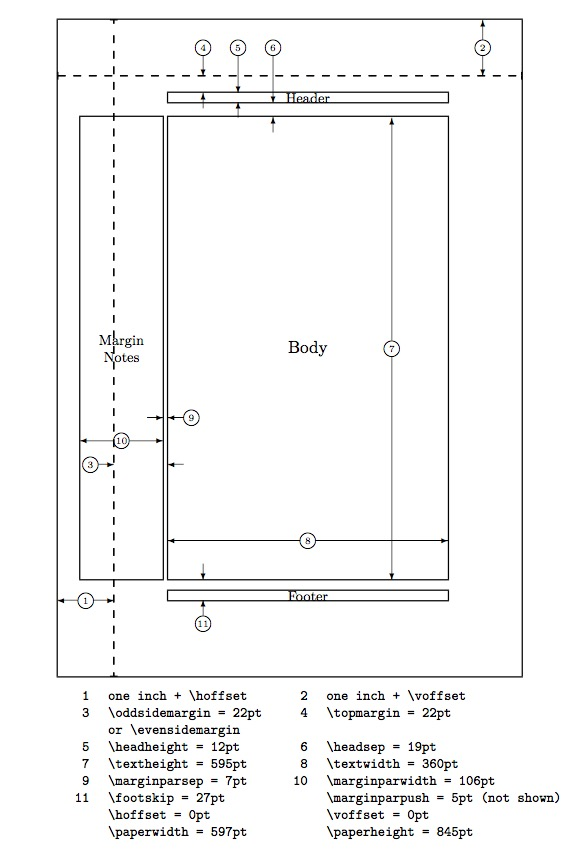
\includegraphics[scale=0.6]{layout.jpg}
    \caption{\zihao{-5}\kaishu \emph{lshort} 一书中的页面布局参数。可以尝试 \texttt{layout} 宏包来打印我们
    自己文档的页面布局。}
    \label{fig:layout}
\end{figure}

\emph{等一下!} 当你欣喜万分,想“不如把这么窄的页面变宽”的时候,先冷静一下。\LaTeX 中大多数东西之所以是那个样子,是
有它们合理的理由的。

的确,和 MS Word 的页面相比,\LaTeX 的页面显得有些窄。但是如果看一下我们喜欢的书籍,并数一数每一行大概有多少字符。然
后你会发现一般每一行的字符数不会超过 66,同样地,\LaTeX 默认的页面布局每一行一般也不超过 66 个字符。经验表明,当一行
文字太长时,阅读起来会变得困难。这是因为一行文字如果太长,人们从这一行的末尾移动到下一行的开头会比较费劲。这也是为什么
报纸要排版成多个竖栏。所以,当我们增加页面的宽度的时候,要考虑到这会使读者的阅读变得困难。

\LaTeX 提供了两种命令来改变页面布局的参数。通常需要在文档的导言区使用这些命令:
\begin{minted}{LaTeX}
    \setlength{parameter}{length}       % 给某个参数设定一个具体的值
    \addtolength{parameter}{length}     % 在某个参数值的基础上增加一定值
\end{minted}

实际上,第二个命令比 \mintinline{LaTeX}{\setlength} 要常用,因为它是在已有设置的基础上改动的。

\subsection{更有趣的长度}
在写 \LaTeX 文档的时候,最好尽可能地避免使用绝对长度。尽量使用一些别的页面元素的长度来替代绝对长度,例如我们想让图片的
宽度铺满页面,就可以使用 \mintinline{LaTeX}{\textwidth} 命令。

下面的三个命令可以让我们决定文本字符串的宽度、高度、深度:
\begin{minted}{LaTeX}
    \settowidth{variable}{text}  % the width of the box
    \settoheight{variable}{text} % the length between the baseline and the top of the box
    \settodepth{variable}{text}  % the length between the baseline and the bottom of the box
\end{minted}

示例代码:
\begin{minted}{LaTeX}
    \newenvironment{vardesc}[1]{
        \settowidth{\parindent}{#1:\ }
        \makebox[0pt][r]{#1:\ }}{}

    \begin{displaymath}
    a^2 + b^2 = c^2
    \end{displaymath}

    \begin{vardesc}{Where}$a$, $b$ -- are adjacent to the right angle of a
        right-angled triangle.

    $c$ -- is the hypotenuse of the triangel and feels lonely

    $d$ -- finally does not show up here at all. Isn't that puzzling?
    \end{vardesc}
\end{minted}

示例输出:
\newenvironment{vardesc}[1]{
    \settowidth{\parindent}{#1:\ }
    \makebox[0pt][r]{#1:\ }}{}

\begin{displaymath}
a^2 + b^2 = c^2
\end{displaymath}

\begin{vardesc}{Where}$a$, $b$ -- are adjacent to the right angle of a
    right-angled triangle.

$c$ -- is the hypotenuse of the triangel and feels lonely

$d$ -- finally does not show up here at all. Isn't that puzzling?
\end{vardesc}

\section{盒子(Boxes)}
\LaTeX 通过盒子来构建页面。首先,每个字母都是一个小盒子,和其他的字母连接起来成为单词。单词又和单词连接在一起成为句
子,但是单词和单词之间的连接是有弹性的,它们之间的空隙可以根据特定的情境来压缩或扩张。

这是一种非常简单的说法,但是却说明了盒子是 \TeX{} 的操作单位。并不仅仅只有字母才能作为盒子,我们几乎可以将任何东西都放
入盒子,包括一些其他的盒子。\LaTeX 在处理时,就会把每个盒子作为一个字母。

之前已经遇到了一些盒子,例如 \texttt{tabular} 环境 和 \mintinline{LaTeX}{\includegraphics} 命令,都会产生盒
子。这意味着我们可以简单地将两个表格或两张图片并排排版,只要确保它们组合在一起后的宽度不超过文本宽度就行了。

我们还可以选定某一个段落,用 \mintinline{LaTeX}|\parbox[pos]{width}{text}| 命令或 \linebreak[7]
\mintinline{LaTeX}|\begin{minipage}[pos]{width} text \end{minipage}| 环境将其放入盒子。其中,\emph{pos}
参数可以设置为 \texttt{c}、\texttt{t} 或 \texttt{b} 来控制盒子的垂直对齐方式。\emph{width} 参数用于指定盒子的
宽度。\texttt{minipage} 和 \mintinline{LaTeX}{\parbox} 的主要区别是,\texttt{parbox} 中不能使用所有的命令
和环境,但是 \texttt{minipage} 中几乎可以任何东西。

\mintinline{LaTeX}{\mbox} 命令只处理水平对齐的内容。它只是把一些盒子打包成另一个盒子,也可以用来防止某两个词被
\LaTeX 打断。由于盒子中可以嵌套盒子,这些水平方向的盒子有很高的灵活性。
\begin{minted}{LaTeX}
    \mbox{text}
    \makebox[width][pos]{text}
\end{minted}
\emph{width} 决定了盒子外框的大小。除了长度表达式以外,还可以在 \emph{width} 参数中使用
\mintinline{LaTeX}{\width}、\mintinline{LaTeX}{\height}、\mintinline{LaTeX}{\depth} 和
\mintinline{LaTeX}{\totalheight},这些值都会从排版的文字获得。\emph{pos} 参数可以是 \texttt{c}(center)、
\texttt{l}(flushleft) 或 \texttt{s}(spread the text to fill the box)。

\mintinline{LaTeX}{\framebox} 和 \mintinline{LaTeX}{\makebox} 很像,但是它会在文本外面画出一个方框。

示例代码:
\begin{minted}{LaTeX}
    \makebox[\textwidth]{c e n t r a l} \par
    \makebox[\textwidth][s]{s p r e a d} \par
    \framebox[1.1\width]{Guess I'm framed now!} \par
    \framebox[0.8\width][r]{Bummer, I am too wide} \par
    \framebox[1cm][l]{never mind, so am I}
    Can you read this?
\end{minted}

示例输出:
\begin{quote}
    \makebox[\textwidth]{c e n t r a l} \par
    \makebox[\textwidth][s]{s p r e a d} \par
    \framebox[1.1\width]{Guess I'm framed now!} \par
    \framebox[0.8\width][r]{Bummer, I am too wide} \par
    \framebox[1cm][l]{never mind, so am I}
    Can you read this?
\end{quote}

前面是如何控制盒子的水平方向特性,而下面的命令可以设置盒子的垂直方向特性。
\begin{minted}{LaTeX}
    \raisebox{lift}[extend-above-baseline][extend-below-baseline]{text}
\end{minted}
在前三个参数中,都可以使用 \mintinline{LaTeX}{\width}、\mintinline{LaTeX}{\height}、
\mintinline{LaTeX}{\depth} 和 \mintinline{LaTeX}{\totalheight} 命令,从而对盒子中的 \emph{text} 产生影
响。

示例代码:
\begin{minted}{LaTeX}
    \raisebox{0pt}[0pt][0pt]{\Large\textbf{Aaaa\raisebox{-0.3ex}{a}%
    \raisebox{-0.7ex}{aa}%
    \raisebox{-1.2ex}{r}%
    \raisebox{-2.2ex}{g}%
    \raisebox{-4.5ex}{h}}}
    she shouted, but not even the next one in line noticed that something
    terrible had happened to her.
\end{minted}

\begin{quote}
    \raisebox{0pt}[0pt][0pt]{\Large\textbf{Aaaa\raisebox{-0.3ex}{a}%
    \raisebox{-0.7ex}{aa}%
    \raisebox{-1.2ex}{r}%
    \raisebox{-2.2ex}{g}%
    \raisebox{-4.5ex}{h}}}
    she shouted, but not even the next one in line noticed that something
    terrible had happened to her.
\end{quote}

\section{Rules}
通常情况下我们用 \mintinline{LaTeX}|\rule[lift]{width}{height}| 来生成一个黑盒子,这在画水平线和垂直线时非常
有用。注意在代码中,如果在行末紧跟着 \texttt{\%},表明这一行未结束,换行就不会产生空格。

示例代码:
\begin{minted}{LaTeX}
    \rule{3mm}{.1pt}%
    \rule[-1mm]{5mm}{1cm}%
    \rule{3mm}{.1pt}%
    \rule[1mm]{1cm}{5mm}%
    \rule{3mm}{.1pt}
\end{minted}

示例输出:
\begin{quote}
    \rule{3mm}{.1pt}%
    \rule[-1mm]{5mm}{1cm}%
    \rule{3mm}{.1pt}%
    \rule[1mm]{1cm}{5mm}%
    \rule{3mm}{.1pt}
\end{quote}

\end{document}
